% ---------------------------------------------------
% Trabajo Final de Grado
% Author: Fabián González Lence <alu0101549491@ull.edu.es>
% Chapter: Arquitectura y Diseño
% ----------------------------------------------------

\chapter{Arquitectura y Diseño} \label{chap:Design}

Este capítulo recoge los artefactos de diseño que sirvieron de entrada al flujo de cuatro fases descrito en el Capítulo~\ref{chap:Metodology}: la especificación de requisitos, los diagramas UML \cite{Fowler:2004:UML} de clases y de casos de uso, las decisiones arquitectónicas y las tecnologías seleccionadas para cada uno de los cinco proyectos. 
Puesto que la caracterización de cada proyecto y la pila tecnológica ya se han presentado en la Tabla~\ref{tab:proyectos-resumen}, el énfasis recae en este Capítulo sobre las decisiones de diseño y su progresión a lo largo del experimento.

\section{Especificación de requisitos} \label{sec:requirements}

La especificación de requisitos se abordó como un experimento en sí mismo, ensayando varios estilos de redacción y varios modelos de \ac{IA} redactores para evaluar cuál ofrecía mejores resultados al alimentar a la \ac{IA} Arquitecto. Se trabajó sobre los niveles de formalización habituales en los lenguajes de especificación de requisitos \cite{Sommerville:2015:SE, Pohl:2010:RE, ISO:29148:2018}: una variante informal centrada en caracterizar la aplicación libremente, una versión semiformal basada en una plantilla estructurada, y un tercer formato que varía entre proyectos: \ac{LNC} en sintaxis \ac{EARS} \cite{Mavin:2009:EARS} para los tres primeros, e Historias de Usuario \cite{Cohn:2004:UserStories} con criterios de aceptación y prioridad para los dos últimos. Todos los documentos de especificación se encuentran versionados en el repositorio del \ac{TFG}\footnote{\href{https://github.com/alu0101549491/TFG-Fabian-Gonzalez-Lence/tree/main/resources/requirement-specifications}{Ficheros de Especificación de Requisitos}}.\\

La especificación semiformal ---introducción, alcance, requisitos funcionales y no funcionales, resumen de actores y arquitectura técnica--- se redactó con ayuda de Claude y constituye la fuente única de verdad para las fases posteriores; la variante informal se derivó de ella para mejorar la caracterización de cara a los modelos generadores de diagramas. Para el tercer formato, Mistral fue el único modelo que produjo una redacción \ac{EARS} con la granularidad y coherencia necesarias, mientras que ChatGPT generó las historias de usuario de \ac{CARTO} y \ac{TENNIS} en formato \textit{HU-XX} con criterios de aceptación y prioridad.\\

El tercer formato varía según la naturaleza del proyecto: el \ac{LNC} en sintaxis \ac{EARS} resultó más adecuado para las aplicaciones autocontenidas de los tres primeros proyectos, mientras que las historias de usuario fueron una traducción más natural de los requisitos en lenguaje cotidiano de clientes reales para \ac{CARTO} y \ac{TENNIS}. En cualquier caso, la especificación semiformal fue el documento de entrada para el Arquitecto. La Tabla~\ref{tab:requirements-count} resume el volumen y los aspectos diferenciadores de cada proyecto.

\begin{table}[H]
\centering
\small
\renewcommand{\arraystretch}{1.3}
\begin{tabularx}{\textwidth}{|>{\raggedright\arraybackslash}p{1.7cm}|>{\raggedright\arraybackslash}p{0.7cm}|>{\raggedright\arraybackslash}p{0.9cm}|Y|}
\hline
\textbf{Proyecto} & \textbf{RF} & \textbf{RNF} & \textbf{Aspectos diferenciadores} \\
\hline
\ac{HANGMAN} & 10 & 8 & Arquitectura \ac{MVC}, diccionario de palabras externalizable \\
\hline
\ac{PLAYER} & 20 & 13 & Reproducción sobre \ac{API} de audio HTML5, arquitectura basada en \textit{custom hooks}, persistencia en \textit{localStorage} \\
\hline
\ac{BALATRO} & 30 & 12 & Evaluador de manos de póker, tres familias de cartas especiales, cinco \textit{Boss Blinds}, economía de tienda \\
\hline
\ac{CARTO} & 30 & 20 & Roles con permisos diferenciados, sincronización tiempo real, integración Dropbox, trazabilidad de auditoría \\
\hline
\ac{TENNIS} & 63 & 19 & Nueve estados de inscripción ITF\footnotemark[1], doce estados de partido, clasificación ELO, notificaciones, ITF/TODS \\
\hline
\end{tabularx}
\caption{Volumen de la especificación de requisitos y aspectos diferenciadores.}
\label{tab:requirements-count}
\end{table}

\footnotetext[1]{Estados ITF: \texttt{OA, DA, SE, JE, QU, LL, WC, ALT, WD}.}

\section{Diagramas de clases y de casos de uso} \label{sec:uml}

A partir de las especificaciones, se generan para cada proyecto los diagramas de clases y los diagramas de casos de uso en formato Mermaid\footnote{\href{https://mermaid.js.org}{Mermaid}}. La colección completa de diagramas intermedios y definitivos se encuentra  en el repositorio\footnote{\textit{See on GitHub}: \href{https://github.com/alu0101549491/TFG-Fabian-Gonzalez-Lence/tree/main/resources/uml-class-diagrams}{Diagramas de Clases} y \href{https://github.com/alu0101549491/TFG-Fabian-Gonzalez-Lence/tree/main/resources/uml-use-case-diagrams}{Diagramas de Casos de Uso}}, organizados por proyecto y por variante de especificación. Ambos diagramas se usan como entrada estructurada para el agente de \ac{IA} Arquitecto, complementando la especificación con una representación formal del dominio y de las interacciones actor-sistema. La elección de Mermaid frente a herramientas más tradicionales se justifica por su versionado en texto plano y, sobre todo, por su capacidad de ser interpretado directamente por los modelos sin necesidad de exportar imágenes.\\

El diagrama de clases describe las entidades del dominio, sus atributos, sus relaciones y la cardinalidad entre ellas. Su complejidad crece de nueve clases en \ac{HANGMAN} a más de cincuenta elementos en \ac{TENNIS} ---entidades, enumeraciones, servicios de aplicación y contratos de repositorio---, reorganizándose en capas de \textit{Clean Architecture} a partir de \ac{CARTO}. La Figura~\ref{fig:hangman-class-diagram} muestra el diagrama definitivo de \ac{HANGMAN}; los diagramas de los proyectos posteriores presentan una complejidad creciente que hace inviable reproducirlos en esta memoria. El diagrama de casos de uso documenta los actores y las interacciones que soportan cada requisito. En los dos primeros proyectos basta un único actor; a partir de \ac{CARTO} aparecen tres roles diferenciados y en \ac{TENNIS} se elevan a cuatro al incorporar al público no registrado como actor de consulta.\\

\begin{figure}[H]
  \centering
  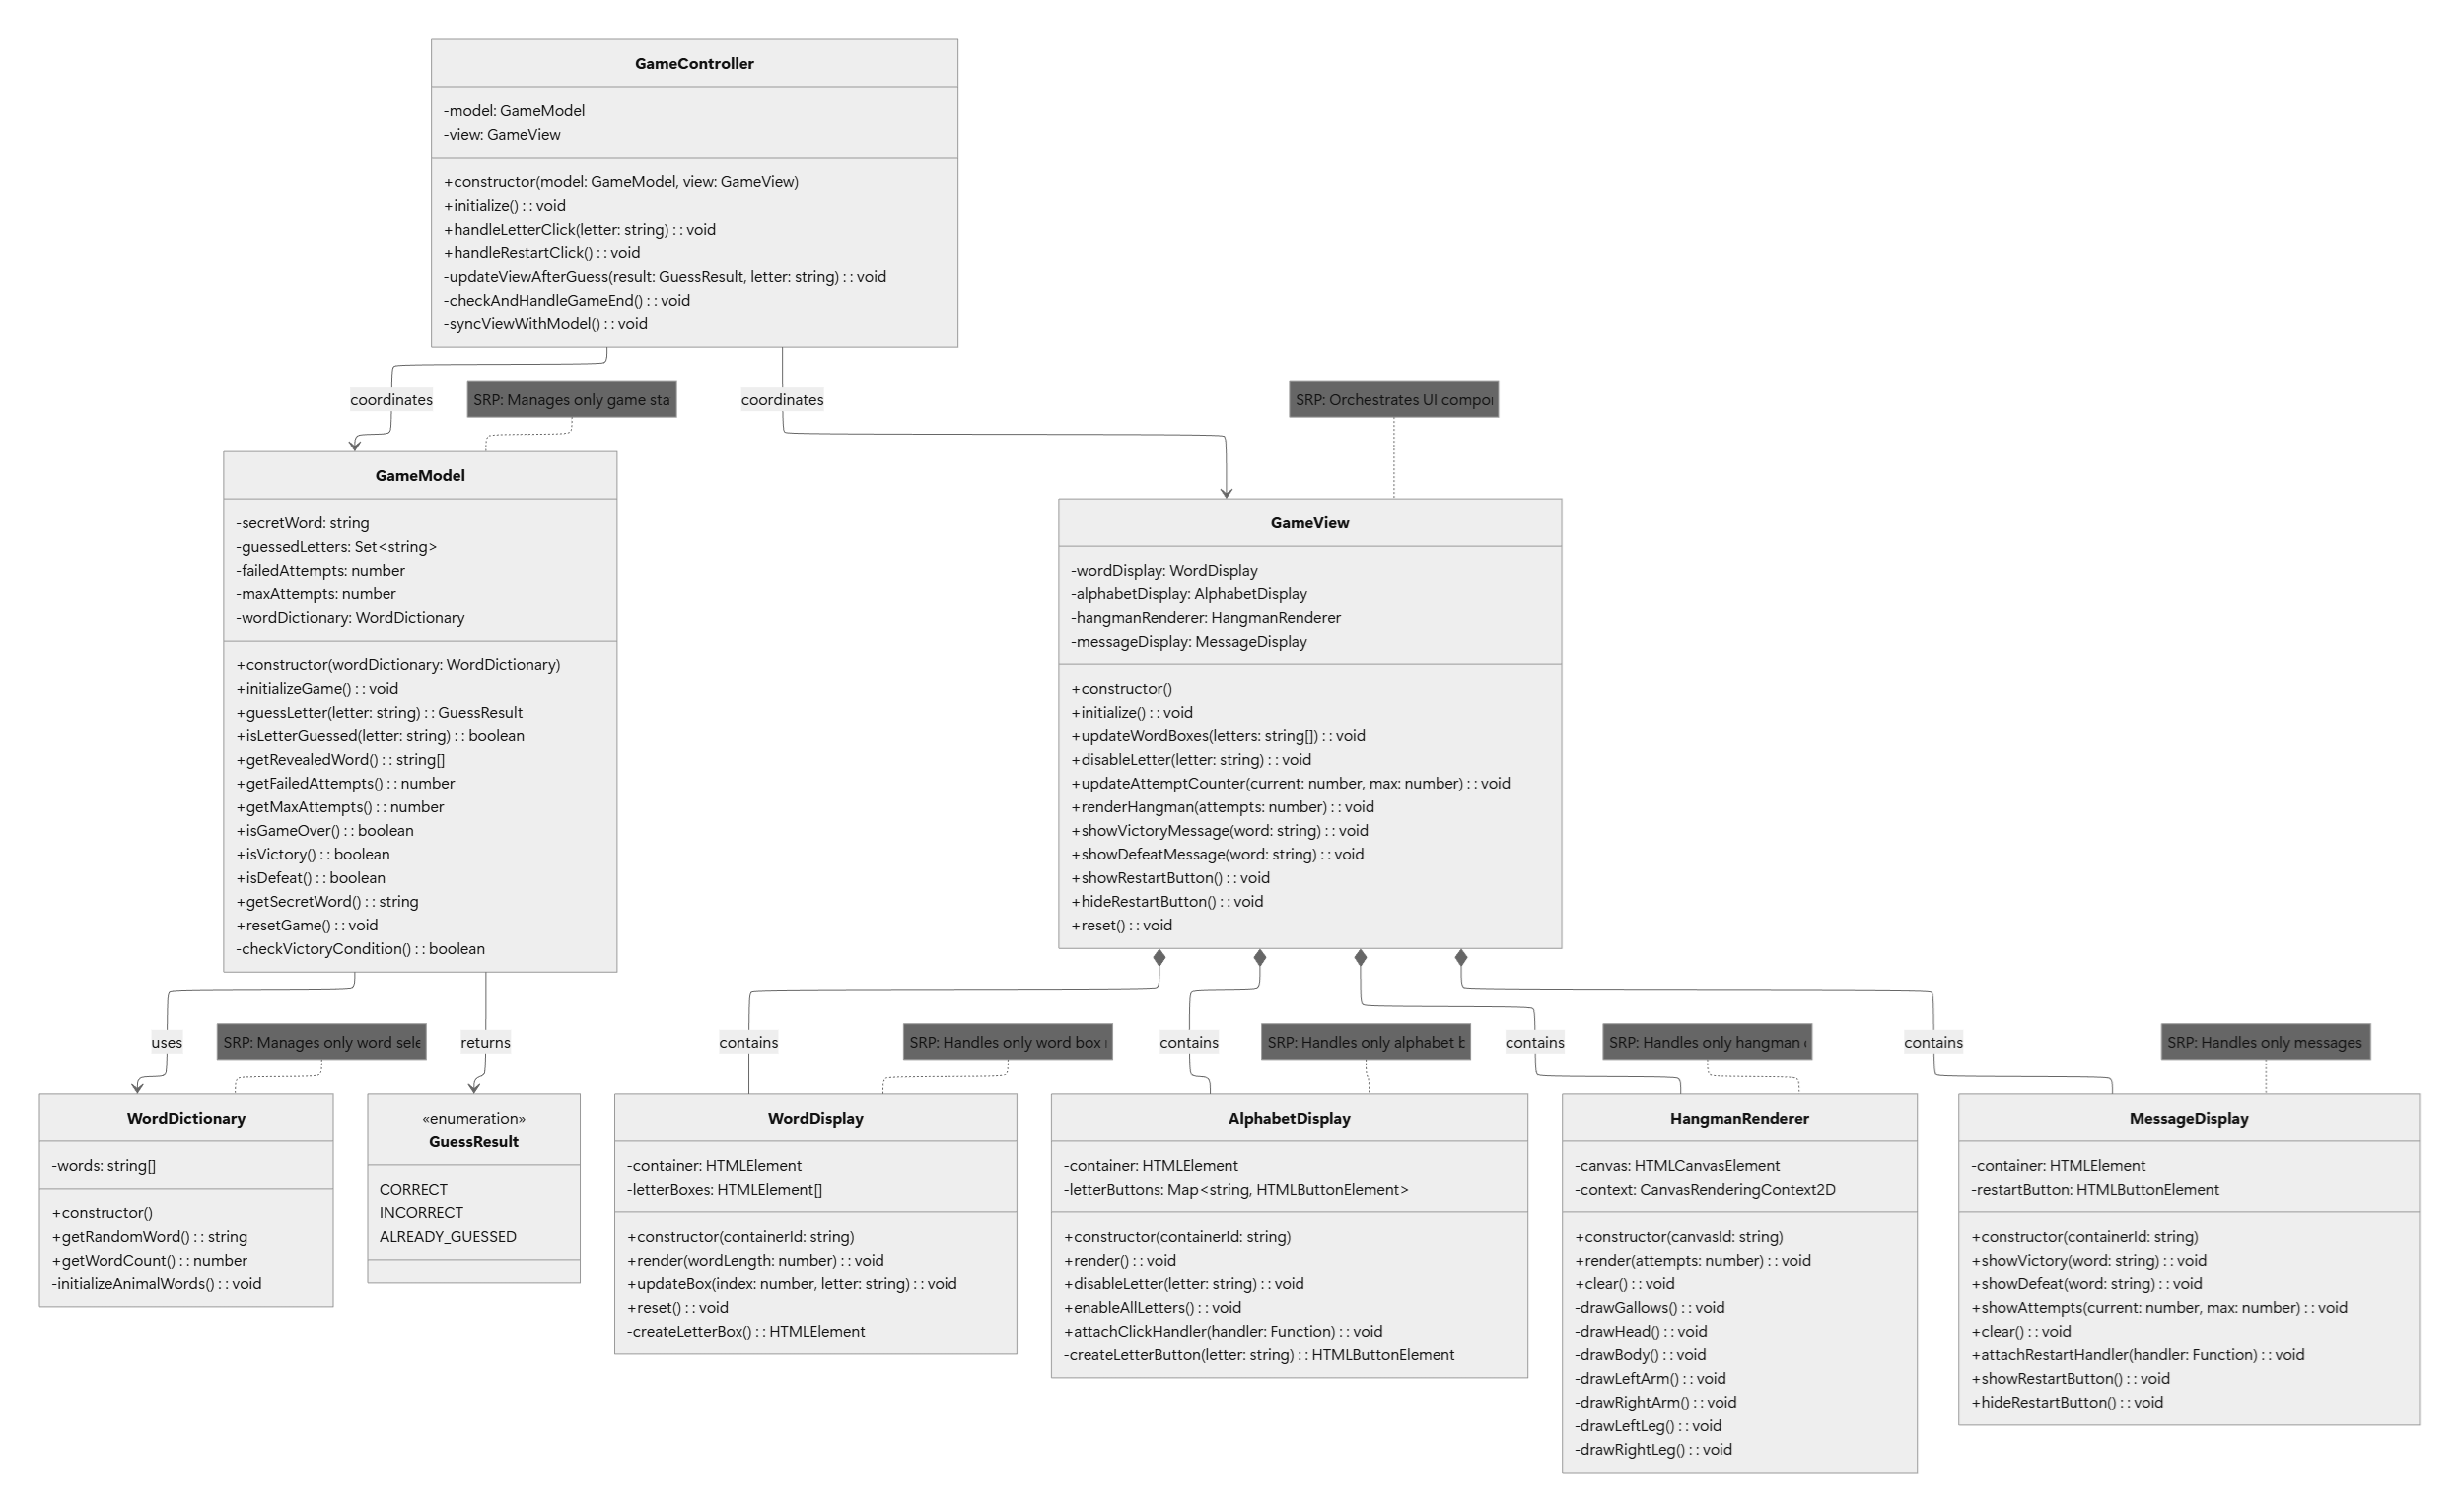
\includegraphics[width=\textwidth]{images/hangman-class-diagram.png}
  \caption{Diagrama de clases UML de \ac{HANGMAN}, generado por Claude a partir de la especificación semiformal. (\textit{\href{https://github.com/alu0101549491/TFG-Fabian-Gonzalez-Lence/blob/main/resources/images/diagrams/}{See on GitHub}})}
  \label{fig:hangman-class-diagram}
\end{figure}

La generación de ambos tipos de diagrama fue un experimento comparativo entre modelos y variantes de especificación: para los diagramas de clases, la variante semiformal produjo resultados más ricos desde el primer intento que la informal, y el \ac{LNC} no aportó ventajas adicionales sobre aquella; para los diagramas de casos de uso, Claude fue el único modelo capaz de generar sintaxis Mermaid válida y fiel a los requisitos, siendo el \ac{LNC} la mejor entrada para P1--P3 y las historias de usuario para P4--P5.

\section{Decisiones arquitectónicas} \label{sec:arch-decisions}

La progresión arquitectónica de los cinco proyectos queda recogida en la Tabla~\ref{tab:proyectos-resumen} y caracterizada en la Sección~\ref{sec:diseno-experimental}; esta sección recoge las motivaciones de cada elección no derivadas del tamaño o la pila tecnológica. \ac{HANGMAN} adopta \ac{MVC} \cite{Reenskaug:1979:MVC} con patrones \textit{Composite} y \textit{Observer} \cite{Gamma:1994:Design} en la vista como línea base deliberadamente conservadora. \ac{PLAYER} pasa a componentes React con \textit{custom hooks} porque el paradigma declarativo impone una separación presentacional-contenedor que el \ac{MVC} no modela con naturalidad. \ac{BALATRO} recupera \ac{MVC} pero añade una capa de servicios transversales para evitar que la lógica de juego absorba responsabilidades ajenas. \ac{CARTO} adopta \textit{Clean Architecture} \cite{Martin:2018:CleanArchitecture} con inversión de dependencias \cite{Martin:2003:Agile}, condición necesaria para el \textit{testing end-to-end}. \ac{TENNIS} replica el mismo esquema \textit{full-stack}, cada extremo con sus propias cuatro capas de \textit{Clean Architecture}, comunicadas por la \ac{API} REST y Socket.io. En todos los proyectos se aplicaron de forma transversal los principios \ac{SOLID} \cite{Martin:2003:Agile} y la guía de estilo de Google.

\section{Pila tecnológica y trazabilidad de decisiones} \label{sec:tech-stack}

La Tabla~\ref{tab:tech-progresion} desglosa las decisiones tecnológicas complementando la Tabla~\ref{tab:proyectos-resumen}. El cambio de \textit{framework} entre proyectos es deliberado —persigue exponer a los modelos a paradigmas distintos— y cada decisión queda registrada en la especificación y reproducida en los \textit{prompts} para evitar que los modelos introduzcan dependencias adicionales por iniciativa propia.

\begin{table}[H]
\centering
\small
\renewcommand{\arraystretch}{1.3}
\begin{tabularx}{\textwidth}{|>{\raggedright\arraybackslash}p{1.8cm}|>{\raggedright\arraybackslash}p{2.2cm}|>{\raggedright\arraybackslash}p{3cm}|Y|>{\raggedright\arraybackslash}p{2.6cm}|}
\hline
\textbf{Proyecto} & \textbf{\textit{Framework} de UI} & \textbf{Gestión de estado} & \textbf{Comunicación con backend} & \textbf{Estrategia de \textit{testing}} \\
\hline
\ac{HANGMAN} & Ninguno & Estado interno & --- & Jest unitario \\
\hline
\ac{PLAYER} & React 18 & \textit{Custom hooks} + \texttt{localStorage} & --- & Jest unitario \\
\hline
\ac{BALATRO} & React 18 & Servicios + \texttt{localStorage} & --- & Jest unitario \\
\hline
\ac{CARTO} & Vue 3 & Pinia & Axios + Socket.io & Playwright \textit{end-to-end} \\
\hline
\ac{TENNIS} & Angular 19 & Servicios Angular + RxJS & \ac{API} REST + Socket.io & Playwright \textit{end-to-end} \\
\hline
\end{tabularx}
\caption{Progresión de decisiones tecnológicas a lo largo de los cinco proyectos.}
\label{tab:tech-progresion}
\end{table}